%!TEX program = xelatex

\documentclass[11pt,titlepage]{report}
%!TEX root = main.tex

\usepackage[T1]{fontenc}
\usepackage{lmodern}
\usepackage[svgnames]{xcolor}
\usepackage{fontspec} % XeLaTeX required!
\usepackage{graphicx}
\usepackage{circuitikz}
\usepackage{tikz}
\usepackage{pifont}
\usepackage[some]{background}
\usepackage{xltxtra} 
\usepackage{setspace}
\usepackage[absolute]{textpos}
\usepackage[latin1]{inputenc}
\usepackage[english]{babel}
\usepackage{graphicx}
\usepackage{wrapfig}
\usepackage{fullpage}
\usepackage[margin=1in]{geometry}
\usepackage{float}
\usepackage{url}
\usepackage{multicol}
\usepackage{hyperref}
\usepackage{titlepic}
\usepackage{standalone}
\usepackage{siunitx}
\usepackage{booktabs}
\usepackage{amsmath}
\usepackage{unicode-math}
\usepackage{verbatim}
\usepackage{enumitem}
\usepackage{listings}
\usepackage{multirow}
\usepackage{pgfplots}
\pgfplotsset{compat=1.8}
\usepackage{caption} 
\usepackage[parfill]{parskip}
\usepackage{import}
\usepackage[backend=bibtexu,texencoding=utf8,bibencoding=utf8,style=ieee,sortlocale=en_GB,language=auto]{biblatex}
\usepackage[strict,autostyle]{csquotes}
\usepackage[final]{pdfpages}
\usepackage{subcaption}
\usepackage{ifplatform}
%\captionsetup[table]{skip=10pt}


% Fix for includepdf bug in Mac OS X
\newcommand{\insertpdfpath}[1]{
	\ifwindows
	\newcommand{\insertpdf}[2]{\includepdf[pages=##1]{##2}}
	\else
	\newcommand{\insertpdf}[2]{\includepdf[pages=##1]{#1/##2}}
	\fi
}

%set fonts
\setmainfont[Ligatures=TeX]{Myriad Pro}
\setmathfont{Asana Math}
\setmonofont{Lucida Console}

\usepackage{titlesec, color}
\renewcommand{\familydefault}{\sfdefault} %set font family
\renewcommand{\arraystretch}{1.2} %set table vertical spacing
\setlength\parindent{0pt} %no paragraph indent
\hypersetup{ %setup hyperlinks
    colorlinks,
    citecolor=black,
    filecolor=black,
    linkcolor=black,
    urlcolor=black
}

%redesign chapter headings
\definecolor{gray75}{gray}{0.75}
\newcommand{\chapternumber}{\thechapter}
\newcommand{\hsp}{\hspace{20pt}}
\titleformat{\chapter}[hang]{\Huge\bfseries}{\chapternumber\hsp\textcolor{gray75}{|}\hsp}{0pt}{\Huge\bfseries}

%Redefine appendix headers
\renewcommand{\appendixname}{Appendix}
\renewcommand{\appendixtocname}{Appendices}
\renewcommand{\appendixpagename}{Appendices}

%For code listings
\definecolor{black}{rgb}{0,0,0}
\definecolor{browntags}{rgb}{0.65,0.1,0.1}
\definecolor{bluestrings}{rgb}{0,0,1}
\definecolor{graycomments}{rgb}{0.4,0.4,0.4}
\definecolor{redkeywords}{rgb}{1,0,0}
\definecolor{bluekeywords}{rgb}{0.13,0.13,0.8}
\definecolor{greencomments}{rgb}{0,0.5,0}
\definecolor{redstrings}{rgb}{0.9,0,0}
\definecolor{purpleidentifiers}{rgb}{0.01,0,0.01}


\lstdefinestyle{csharp}{
language=[Sharp]C,
showspaces=false,
showtabs=false,
breaklines=true,
showstringspaces=false,
breakatwhitespace=true,
escapeinside={(*@}{@*)},
columns=fullflexible,
commentstyle=\color{greencomments},
keywordstyle=\color{bluekeywords}\bfseries,
stringstyle=\color{redstrings},
identifierstyle=\color{purpleidentifiers},
basicstyle=\ttfamily\small}

\lstdefinestyle{c}{
language=C,
showspaces=false,
showtabs=false,
breaklines=true,
showstringspaces=false,
breakatwhitespace=true,
escapeinside={(*@}{@*)},
columns=fullflexible,
commentstyle=\color{greencomments},
keywordstyle=\color{bluekeywords}\bfseries,
stringstyle=\color{redstrings},
identifierstyle=\color{purpleidentifiers},
}

\lstdefinestyle{matlab}{
language=Matlab,
showspaces=false,
showtabs=false,
breaklines=true,
showstringspaces=false,
breakatwhitespace=true,
escapeinside={(*@}{@*)},
columns=fullflexible,
commentstyle=\color{greencomments},
keywordstyle=\color{bluekeywords}\bfseries,
stringstyle=\color{redstrings},
identifierstyle=\color{purpleidentifiers}
}

\lstdefinestyle{vhdl}{
language=VHDL,
showspaces=false,
showtabs=false,
breaklines=true,
showstringspaces=false,
breakatwhitespace=true,
escapeinside={(*@}{@*)},
columns=fullflexible,
commentstyle=\color{greencomments},
keywordstyle=\color{bluekeywords}\bfseries,
stringstyle=\color{redstrings},
identifierstyle=\color{purpleidentifiers}
}

\lstdefinestyle{xaml}{
language=XML,
showspaces=false,
showtabs=false,
breaklines=true,
showstringspaces=false,
breakatwhitespace=true,
escapeinside={(*@}{@*)},
columns=fullflexible,
commentstyle=\color{greencomments},
keywordstyle=\color{redkeywords},
stringstyle=\color{bluestrings},
tagstyle=\color{browntags},
morestring=[b]",
  morecomment=[s]{<?}{?>},
  morekeywords={xmlns,version,typex:AsyncRecords,x:Arguments,x:Boolean,x:Byte,x:Char,x:Class,x:ClassAttributes,x:ClassModifier,x:Code,x:ConnectionId,x:Decimal,x:Double,x:FactoryMethod,x:FieldModifier,x:Int16,x:Int32,x:Int64,x:Key,x:Members,x:Name,x:Object,x:Property,x:Shared,x:Single,x:String,x:Subclass,x:SynchronousMode,x:TimeSpan,x:TypeArguments,x:Uid,x:Uri,x:XData,Grid.Column,Grid.ColumnSpan,Click,ClipToBounds,Content,DropDownOpened,FontSize,Foreground,Header,Height,HorizontalAlignment,HorizontalContentAlignment,IsCancel,IsDefault,IsEnabled,IsSelected,Margin,MinHeight,MinWidth,Padding,SnapsToDevicePixels,Target,TextWrapping,Title,VerticalAlignment,VerticalContentAlignment,Width,WindowStartupLocation,Binding,Mode,OneWay,xmlns:x}
}

\lstdefinestyle{matlab}{
language=Matlab,
showspaces=false,
showtabs=false,
breaklines=true,
showstringspaces=false,
breakatwhitespace=true,
escapeinside={(*@}{@*)},
columns=fullflexible,
commentstyle=\color{greencomments},
keywordstyle=\color{bluekeywords}\bfseries,
stringstyle=\color{purpleidentifiers},
identifierstyle=\color{purpleidentifiers}
}

%defaults
\lstset{
basicstyle=\ttfamily\small,
extendedchars=false,
numbers=left,
numberstyle=\ttfamily\tiny,
stepnumber=1,
tabsize=4,
numbersep=5pt
}
\addbibresource{../../library/bibliography.bib}

\begin{document}

\chapter{Assignment 1}
\section{Labday 1}
\subsection{Report 1}
\begin{figure}[H]
	\centering
	\usetikzlibrary{shapes,arrows}
\tikzstyle{block} = [
	rectangle,
	draw,
	fill=blue!20, 
    text width=7em, 
    text centered,
    rounded corners,
    minimum height=4em
]
\tikzstyle{every edge} = [
	draw,
	>=triangle 90
]

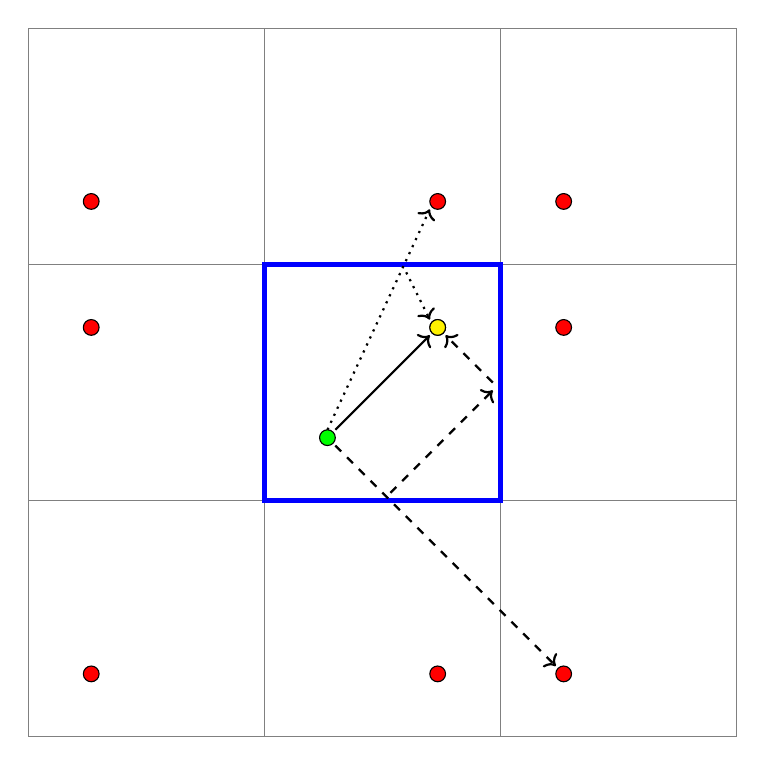
\begin{tikzpicture}[node distance = 5cm, auto]
	% grid
	\draw[step=3cm,gray,thin] (0,0) grid (9,9);
	\draw[draw=blue,ultra thick] (3,3) rectangle (6,6);

	% transmitter
	\filldraw[fill=green] (3.8,3.8) circle (1mm);
	% receiver replicas
	\foreach \x in {0.8,5.2,6.8}
		\foreach \y in {0.8,5.2,6.8}
			\filldraw[fill=red] (\x,\y) circle (1mm);
	% receiver
	\filldraw[fill=yellow] (5.2,5.2) circle (1mm);

	% lines
	% straight
	\draw[thick,->,draw=black] (3.9,3.9) -- (5.1,5.1); 
	% one reflection
	% \draw[thick,->,draw=black,dotted] (3.6,3.9) -- (0.9,5.1);
	% \draw[thick,->,draw=black,dotted] (3.1,4.2) -- (5.1,5.1);
	% one reflection
	\draw[thick,->,draw=black,dotted] (3.8,3.9) -- (5.1,6.7);
	\draw[thick,->,draw=black,dotted] (4.8,5.9) -- (5.1,5.3);
	% two reflections
	\draw[thick,->,draw=black,dashed] (3.9,3.7) -- (6.7,0.9);
	\draw[thick,->,draw=black,dashed] (4.6,3.1) -- (5.9,4.4);
	\draw[thick,->,draw=black,dashed] (5.9,4.5) -- (5.3,5.1);

\end{tikzpicture}
	\caption{Some possible reflections}
	\label{fig:reflections}
\end{figure}
Given a square room confined by the blue lines in figure \ref{fig:reflections} with a sound source depicted by the green dot and a microphone depicted by the yellow dot, it is easy to calculate the number of reflections heard at the yellow dot by reflecting the room about each wall. If the number of reflections is one, the result is that each wall must be mirrored once and the result is figure \ref{fig:reflections} excluding the four corner rooms, for a total of five reflections (no reflection + 4 reflections). The red dots in the reflected rooms represent the yellow dot as projected through the wall. After 2 reflections, figure \ref{fig:reflections} should be extended by four more rooms, yielding 13 reflections.

To see the impulse response of the room with two reflections we made use of the \texttt{MATLAB} script provided in appendix ... The impulse response is shown in figure ...
We extended the \texttt{MATLAB} model to incorporate an arbitrary amount of reflections. The resulting room diagram is shown in figure ... and the resulting impulse response is shown in figure ...
\subsection{Report 2}
%corresponding matlab file: resource/labday1/report2.m
The impulse response for $a=0.95$ and $a=-0.95$ is shown in figure .. For $a=0.95$ the filter causes a damped oscillation, for $a=-0.95$ it causes an exponentially decaying signal.

The frequency domain plots are shown in figure ... It can be seen that for $a=0.95$ the filter behaves as a band pass filter and for $a=-0.95$ it behaves as a band stop filter.

There is no \texttt{MATLAB} function for the FT or DTFT because these produce continuous results and \texttt{MATLAB} is a numerical package which can't handle that.
\subsection{Report 3}



\subsection{Report 4}
%Corresponding matlab file: resources/labday1/report4.m
Figure ? shows a heatmap of the occurrence of frequencies in \SI{20}{\milli \second} intervals of the standard \texttt{MATLAB} train soundbyte. It is apparent that most of the sound is centered around \SI{10}{\kilo\hertz}. The two whistle blows are also clearly distinguishable. 

\subsection{Report 5}
Zero padding
\subsection{Report 6}
extended zero padding
\subsection{Report 7}
Convolution property p.95

\end{document}